\documentclass[12pt]{article}
\renewcommand{\contentsname}{Inhalt}
\usepackage{graphicx}
\usepackage[margin=25mm]{geometry}
\usepackage{multicol}
\usepackage[
backend=biber,
style=numeric,
sorting=nyt,
defernumbers=false
]{biblatex}
\usepackage{hyperref}
\hypersetup{
    colorlinks=true,
    linkcolor= black,
    filecolor=black,      
    urlcolor=black,
    pdftitle={NN Graph Classifier},
    pdfpagemode=FullScreen,
    citecolor=black,
    linktoc=all,
    pdfnewwindow=true,
    pageanchor=true,
    }

\graphicspath{ {./imgs/} }

\addbibresource{References.bib}

\title{NN Portfolio Optimierung}
\date{09. Februar 2024}
\author{Patrick Spohr}

% Line spacing
\linespread{1.5} 

\begin{document}

    \renewcommand{\figurename}{Visual}
    \renewcommand{\tablename}{Visual}

    \begin{titlepage}
        
        \centering
        \Huge \textbf{Neural Network Graph Classifier}

        \vspace{7mm}
        
        \centering
        \Large \textit{of Probability Distributions} 

        \vspace{7mm}

        \centering
        \large by

        \vspace{7mm}

        \large Patrick Spohr
        \vspace{2mm}
        \\ 20th February 2024

        \vspace{10mm}

        \centering
        \large Code
        \vspace{1mm}
        \\ \normalsize \textit{https://github.com/p-spohr/NN-Graph-Classifier} 
        
        \vspace{20mm}

        \centering
        \large Master’s Program
        \vspace{1mm}
        \\ \normalsize \textit{Finanzmathematik, Aktuarwissenschaften und Risikomanagement} 

        \vspace{5mm}

        \centering
        \large Department
        \vspace{1mm}
        \\ \normalsize \textit{Informatik, Kommunikation und Wirtschaft} 

        \vspace{5mm}

        \centering
        \large Course 
        \vspace{1mm}       
        \\ \normalsize \textit{Deep Learning Seminar} 

        \vspace{5mm}

        \centering
        \large Professor
        \vspace{1mm}
        \\ \normalsize \textit{Dr. Alla Petukhina} 


    \end{titlepage}

    \hypertarget{Table of Contents}{\tableofcontents}

    \newpage

    \newpage \section{Motivation and Objectives} 
    
        \subsection{Graph Classifier}
            
            In the age of information, those that can successfully and quickly interpret large amounts of data will have an advantage. 
            The field where converting data into visual aids is called descriptive statistics
            and the most common method to do this is with graphs. 
            This follows the adage, ''A picture says a thousand words.'' 
            With just a glance someone can understand and make connections about the data without needing to scan through a table of numbers. 
            There are many different kinds of graphs: bar charts, pie, charts, line graphs, scatter plots, 
            and radar charts to name a few. Within those charts they can be divided up into more types, 
            like stacked bar charts or donut charts. 
            From science to business charts are the main way key parts of the data are shown to other researchers, customers, or investors. 

            The McDonald’s 2022 Annual Report \cite{mcdonalds2022} has a total of 73 pages and 8 graphs. 
            Each graph displays important information to the investor, like the figure which shows total revenues by segment on page 13. 
            One can see that from 2020 to 2022 the revenue from international operated markets rose and fell, but overall, 
            the revenue share from the different segments have remained static. 
            Wouldn’t it be beneficial to have access to these graphs immediately without needing to browse through the whole report? 
            The ability to identify and then classify graphs instantly in the report without needing to read through it 
            and snip out the graphs manually would save time and effort. The overall flow of this system would have three parts: 
            Identify, Locate, and Organize. Identify would simply see if it is a graph or not and classify it into a type of graph. 
            Once that is finished then the graphs can be located on a page and extracted. 
            The last part would organize the charts for easy viewing. My focus is on the Identify part of this system and will be limited to building a model that answers two questions: Is this image a graph? What kind of graph is it? Regarding the second question, I’ll limit the scope even further because of the multitude of different graphs. The focus will be on classifying the probability distribution in a graph. This was chosen because of the novelty of the problem – no similar projects were found – and because of my current study of stochastics.
        
            
        \subsection{Literature Review}  

            I’ll need to briefly mention the literature I tried to find and the literature that guided this project. 
            As mentioned earlier, this project is quite novel in its end goal 
            since I did not find any research that specifically tried to classify graphs into probability distributions. 
            There were projects that classified graphs into bar charts, pie charts, etc., but even then, 
            those projects were not part of published research. 
            When one tries to search for a neural network graph classifier 
            or a similar pattern the first results are about Graph Neural Networks or GNNs, 
            which are unrelated. As for image classification itself, there are a plethora of papers and resources. 
            I personally learned a lot from a Stanford University course \cite{cs231n2023} 
            and \textit{An Introduction to Convolutional Neural Networks} from O’Shea and Nash \cite{oshea2015}.


        \subsection{Main Goals}

            As stated previously, my focus is on the identification and classification of graph images. 
            This can be accomplished in two types of models where the first one classifies a graph image from a natural image (non-graph) 
            and the second one classifies a graph image into its probability distribution. 
            There are many probability distributions to choose from, but I selected the normal distribution, 
            log-normal distribution, exponential distribution, and uniform distribution. 
            I primarily choose these distributions because they are common and relatively distinct from each other. 
            The reasoning behind this two-model process is to be able to produce a baseline result 
            where it is known that graphs can be distinguishable from natural images. 
            I predicted early on that graphs would be quite distinguishable from natural images and the accuracy of this model would be high, 
            but as it will be discussed later, there is a second component to this problem specific to my data. 
            These hurdles will be expanded upon in the next section.

            In summary, the workflow of the project was split into four steps: 
            get data, create graph classifiers, create distribution classifiers, and evaluate the models. 
            Getting data had the potential to be the hardest step of this project 
            because of the novelty of its goals to classify graph images into their probability distributions 
            and I was partly correct. The next major obstacle was choosing the right model to build the machine learning models 
            and the method in which each image would be classified.  
            In the “Methods” section, I will go in depth to explain the process of how the models were built and the images classified.
        
        
        \subsection{Initial Problems}
        
            As image classification is a vibrant and bustling field, 
            there is no shortage of natural images of various types of things 
            -- cars, airplanes, horses, cats, dogs, clothes, etc. 
            One of the most common datasets for natural images is the CIFAR-10 \cite{ krizhevsky2009} 
            as it is well labeled and contains various images. The task of finding graph images was much more difficult. 
            However, there was a suitable dataset of graphs on Kaggle from SunEdition \cite{sunedition2021} 
            which met my requirements to build the first model, which simply classifies an image as a graph or not a graph. 
            Unfortunately, this dataset does not contain classes with specific probability distributions 
            and cannot be used for the second model -- classifying the four chosen distributions in graphs.

            The biggest issue was getting a dataset with the normal distribution (norm), log-normal (lognorm) distribution, 
            exponential distribution (exp), and uniform distribution (unif) as its four classes. 
            As I saw it, this could be solved in two possible ways. 
            First, I could have scraped the graphs from various online sources. 
            This leads to a major issue of not only where to scrape the graphs but how to label them time efficiently. 
            The dataset from SunEdition on Kaggle has some major drawbacks when wanting to classify the images into more specific classes. 
            These would be apparent in my own scraped graphs as well. Many graphs have more than one graph type in the image. 
            That makes the correct classification impossible. Additionally, the dataset includes ‘graph-like’ images 
            which are depictions of graphs but have no numerical value and are closer to art or natural images. 
            I could also mention that even in a graph type, like bar charts, there are subcategories -- stacked bar charts, 
            horizontal bar charts, vertical bar charts, etc. 
            Were I try to scrape the graphs, then I would lose control of the variables 
            and spend most of my time labeling each graph which would be impossible for the timeframe of the project. 
            This leads to the second solution to my problem. I could generate the graphs.
        
            Generating graphs with the aid of a graphing library was the most time effective solution to acquire thousands of graphs 
            with the four distributions in already-labeled classes. 
            This is not the ideal solution since it biases the dataset towards the design conventions of the chosen graphing library 
            and it lacks the variety seen online, but it can be highly randomized to mimic the potential graphs in various sources 
            and the variables can be controlled to ensure all graphs have the potential to be classified. 
            The most important consideration in this method is the time saved by generating the graphs. 
            The daunting task of scraping and labeling 10,000 graphs can now be minimized into writing a script using a graphing library. 
            The specifics of the three datasets used will be further explained in the subsequent section.
        
        
    \section{Data}
            
        \subsection{CIFAR-10 Images}
        
            \begin{table}[h]
            
                \begin{center}

                    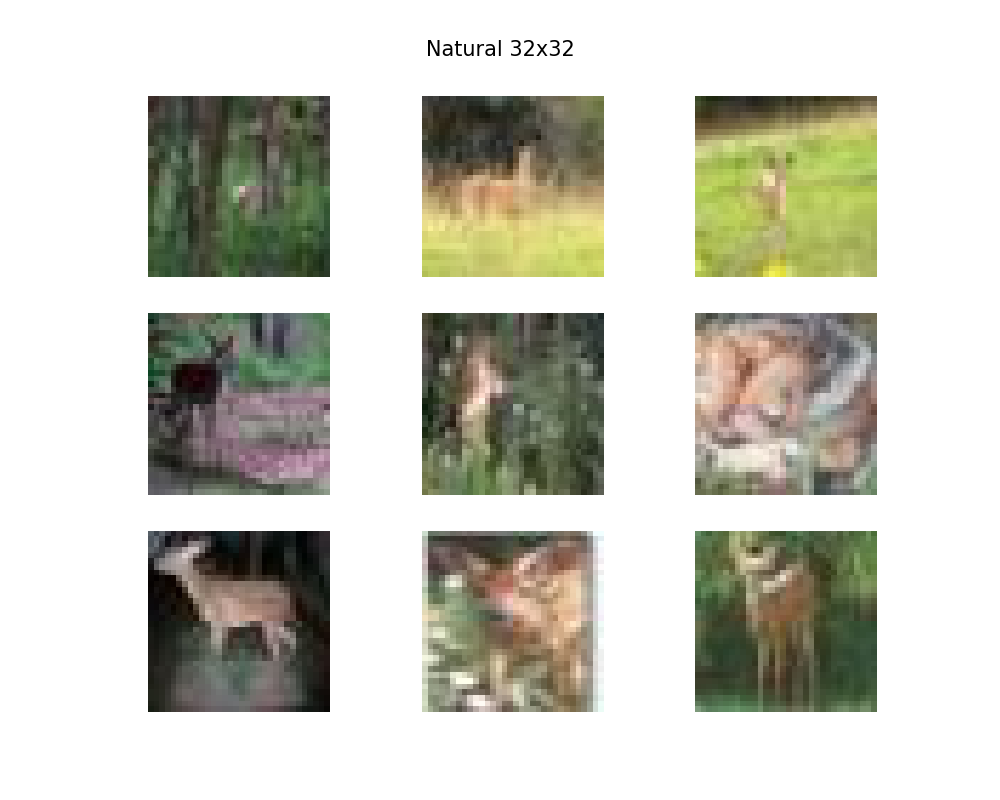
\includegraphics[scale=0.6]{natural_overview.png}
                    \caption{CIFAR-10 Natural Images (CIFAR) Deer Examples \cite{krizhevsky2009}}
                    \label{cifar-overview}
        
                \end{center}
                
            \end{table}

            The CIFAR in CIFAR-10 stands for the Canadian Institute for Advanced Research and the 10 represents the 10 classes in the dataset: 
            airplane, automobile, bird, cat, deer, dog, frog, horse, ship, and truck \cite{krizhevsky2009}. 
            The data comes in six batches of 10,000 images with a total of 60,000 images. 
            The 10,000 images in each batch are made up of 10 classes with 1,000 images per class. 
            The images are colored and 32x32, which means they have a shape of (32,32,3). 
            The first two values represent the dimensions and the 3 stands for the red, green, and blue channels. 
            This data structure is known as a tensor. However, the original data type is a flat NumPy array of (3072,), 
            so each image needed to be reshaped to fit in the model with the graphs.
            

            The updated dataset has 10,000 images (first-batch) that are all 32x32 and in JPG format. 
            Also, the 10 classes have been combined into one natural image class. 
            I have only selected 10,000 because there are only 7,753 suitable graphs in the scraped graph dataset. 
            Had I selected more that would have led to an imbalanced dataset in the model. 
            In my project, the CIFAR-10 dataset will be labeled as CIFAR or natural. See Figure \ref{cifar-overview} for examples.


            
        \subsection{Scraped Graphs}
    
            Just like the CIFAR-10 dataset, the scraped dataset \cite{sunedition2021} needed to get updated to work 
            with the simple graph classifier model as well. The original dataset has 15,786 images and 8 classes. 
            The classes are just image, bar chart, diagram, flow chart, graph, growth chart, pie chart, table. 
            As you can see ‘just image’ refers to non-graphs or natural images, so it needed to be removed. 
            Other classes like table, flow chart, and growth chart were not necessary and were removed as well.

            In the end, four classes were kept, bar chart, diagram, graph, and pie chart, 
            so the total images now used were 7,753. 
            he images came in various dimensions and were resized to the natural images 32x32 and converted to JPG format. 
            I’ll note here that JPG was chosen because it only has 3 color channels and no alpha channel. 
            If PNG is used then it could have a shape of (32,32,4) which adds unnecessary parameters for the scope of my objectives.
            See Visual \ref{scraped-overview} for examples.
            

            \begin{table}[h]
            
                \begin{center}

                    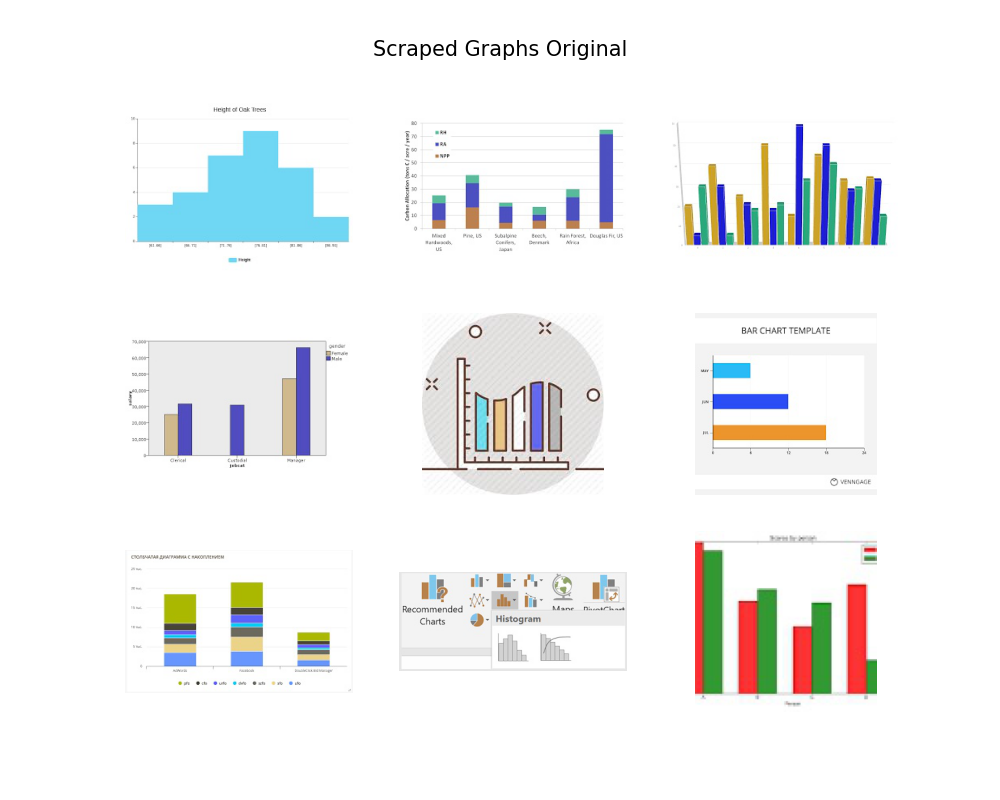
\includegraphics[scale=0.6]{scraped_overview_original.png}
                    \caption{Scraped Graphs (SCP) Bar Chart Examples \cite{sunedition2021}}
                    \label{scraped-overview}
        
                \end{center}
                
            \end{table}

            

        \subsection{Generated Graphs}
            
            \begin{table}[h]
                
                \begin{center}

                    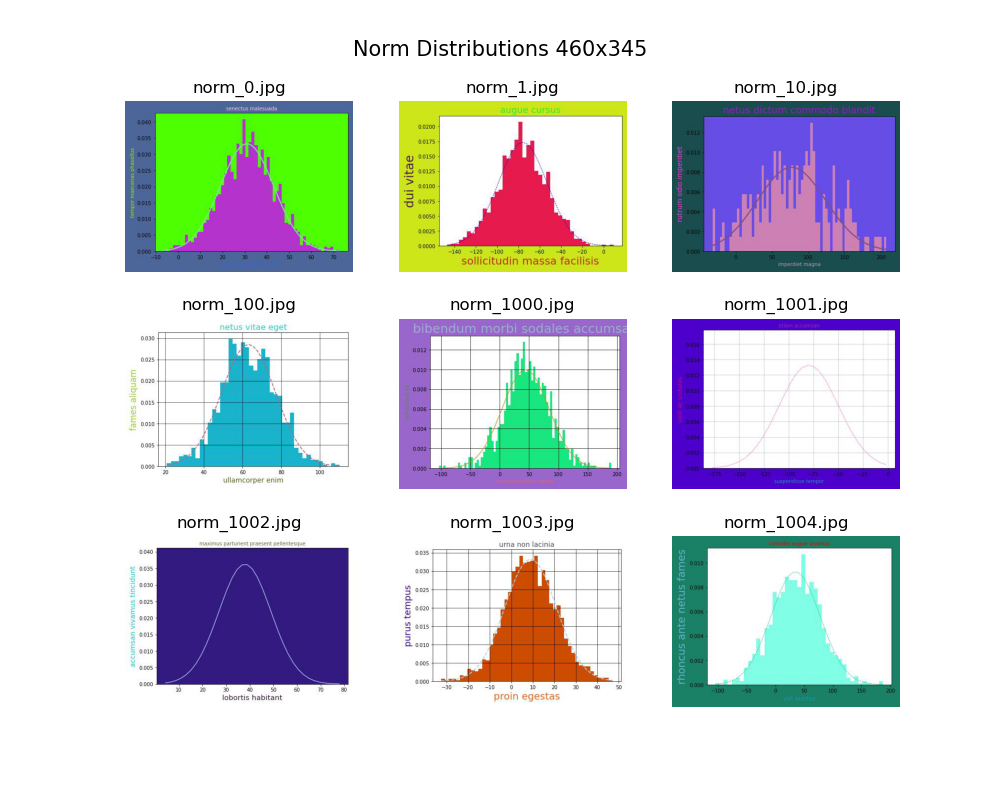
\includegraphics[scale=0.6]{norm_460x345_overview.png}
                    \caption{Generated Graphs (GEN) Normal Distribution Examples}
                    \label{generated-overview}
        
                \end{center}
                
            \end{table}

            Lastly, 8000 graphs were generated in a 460x345 dimension and JPG format. 
            The graphing library used was Matplotlib in Python, 
            but I’ll discuss the programs and libraries in more detail in the “Methods” section. 
            There were 4 classes -- norm, lognorm, exp, and unif -- with 2,000 images each. 
            The only thing updated were the dimensions which included 32x32, 115x86, and 153x115. 
            For clarity, these dimensions follow the Windows format of width by height.

            As for the design, almost every part of the graph was randomized. 
            The color of the histogram bars, line, figure color (outside the box), face color (inside the box where the plot is), 
            and text labels were changed, but the figure color and face color were biased to white by 20 percent 
            because most graphs tend to be white. There was also some changes to ensure 
            that the histogram bars, line, and face don’t have the same color. 
            Regarding the histogram and line, both were visible or only one was visible. 
            The line style was solid or a dash. Each graph had a title, y label, and x label which consisted of lorum ipsum, 
            which is Latin gibberish and is commonly used in web design. 
            The idea behind this was to avoid a bias to English if someone used this model to predict graphs with different languages. 
            The text also had randomized size. Lastly, the density function parameters were randomized 
            to ensure many variations of each probability distribution. 
            
            Overall, the graphs looked like something that could be found in a report, book, or online. 
            The biggest issue with the generated graphs were the so-called ‘duds’ which looked blank because the color of the face, 
            histogram, and line were too similar. This wasn’t a large amount of images, 
            so I decided to keep them instead of manually deleting all of them. 
            I reasoned that keeping the original generated the same is better for reproducibility, 
            rather than someone, me, deciding if a graph is a dud or not since some graphs are on the border of being a dud or not. 
            Ultimately, the seed of the graph generator remains the same and the dataset can always be recreated and used in the model.
            
            Early on, I pre-identified possible misclassifications once I scanned through the set of generated graphs. 
            The similarities between some of the graphs, especially the log-normal and normal distribution, were considerable. 
            They were not ‘duds’ like previously mentioned -- they looked typical, but because of the density functions’ parameters, 
            they were similar in appearance to a point where it would become a 50-50 decision if I had to classify them myself. 
            The cases when this happened are a minority, but it was important to keep this in mind as I evaluated the models later.
            See Visual \ref{generated-overview} for examples. The density functions that created the random variables in the graph
            are listed below.
            

            \textbf{Normal Distribution Density Function  $ X \sim \mathcal{N}(\mu, \sigma^2)  $}
               
            \begin{Large} 

                \[ f_X(x) = \frac{1}{\sqrt{2\pi \sigma^2}} exp\left[{-\frac{(x - \mu)^2}{2 \sigma^2}}\right] \] 

            \end{Large}

            \textbf{Log-Normal Distribution Density Function  $ X \sim L\mathcal{N}(\mu, \sigma^2) $}

            \begin{Large} 

                \[ f_X(x) = \frac{1}{\sqrt{2\pi \sigma^2}} exp\left[{-\frac{(log(x) - \mu)^2}{2 \sigma^2}}\right] \] 

            \end{Large}

            \textbf{Exponential Distribution Density Function  $ X \sim \textnormal{Exp}(\lambda) $}

            \begin{Large} 

                \[ f_X(x) = \lambda exp(- \lambda x) \] 

            \end{Large}
            
            \textbf{Uniform Distribution Density Function  $ X \sim \textnormal{U}[a, b] $}
            
            \begin{Large} 

                \[ f_X(x) = \frac{1}{b - a} \] 

            \end{Large}

    \newpage \section{Methods}

        \subsection{Overview}

            As an introduction to the methods used, I’ll briefly list the steps taken to achieve my objectives. 
            Firstly, I reviewed literature available on artificial neural networks or ANNs and convolutional neural networks 
            or CNNs and then I familiarized myself with TensorFlow, Keras, and Pillow (Python library for images). 
            After that I found natural images (CIFAR) and scraped images (SCP). 
            The next step was generating the graph dataset (GEN) in 32x32, 115x86, 153x115 dimensions. 
            With all the data prepared, I trained simple graph classifiers using CIFAR, SCP, GEN datasets using 32x32 images. 
            Those models were then evaluated by using saved Keras model to predict the images. 
            Subsequently, I moved on to train the distribution graph classifiers using 32x32, 115x86, 153x115 dimensions. 
            In order to see where the models of the distribution classifier models misclassified, 
            I input all the images into the saved Keras models again. 
            Lastly, I tested untrained images with the distribution classifier 153x115 which were not used in any model previously.
        
        \subsection{Feed-Forward Neural Networks}

            The ANN process used in my model is called a feed-forward neural network or FNN. 
            The structure of the model consists of three parts and are shown in Visual \ref{nn-bishop}: 
            an input layer, one or many hidden layers consisting of neurons, and an output layer. 
            The two main processes in the model are forward-propagation and back-propagation, 
            and can be summed up by their respective goals, producing an estimate and minimizing the loss. 
            Forward-propagation begins once the model is built and the data is split into the input values x and the target values y. 
            In this scenario the goal is to use x to predict y.  

            The input data starts from the input layer and flows into the neurons in the hidden layers where it gets multiplied by a weight. 
            The process can be defined as the dot product between the input values and their respective weights. 
            The product then goes into an activation function in the neuron 
            so that the neuron ‘fires’, returning a modified value, or ‘rests’ -- gives zero. 
            The process is repeated through every hidden layer until the output value from the final hidden layer enters the output layer, 
            where it is again put into an activation to determine the final prediction or estimate. 
            The estimate is then put into a loss function to calculate the loss or difference between the estimate and target value. 
            From here a process called back-propagation starts which goes from the back to the front of the entire model. 
            The loss function gets minimized by an optimizer using gradient descent to achieve the smallest possible loss 
            and this is done by changing the weights between the neurons for every layer and every connection. 
            Forward-propagation and back-propagation are repeated until the loss is minimized enough to suit the goal of the model.
        
            
            \begin{table}[h]
            
                \begin{center}

                    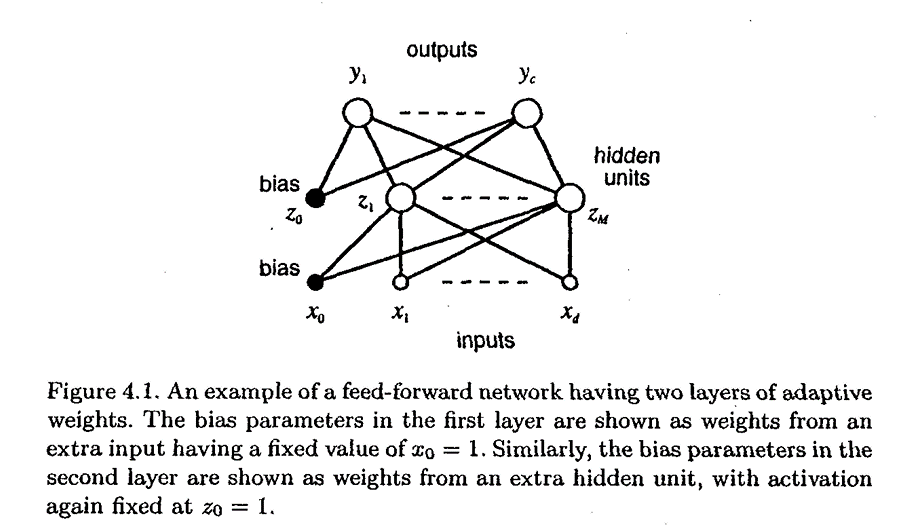
\includegraphics[scale=1]{neural-network-bishop.png}
                    \caption{Neural Network \cite{bishop1995}}
                    \label{nn-bishop}
        
                \end{center}
                
            \end{table}

          

        \subsection{Convolutional Neural Networks}

           \subsubsection{CNNs vs. FNNs}

            
                In order to classify images, the FNN model needs to be adjusted to take the tensor shape of images into account. 
                This is where convolutional neural networks or CNN come into play. 
                The biggest difference between convolutional neural networks 
                or CNNs and a more standard FNN is that they are mostly used in image classification. 
                CNNs enable encoded image-specific features into the architecture (location + color), 
                making the network more suited for image-focused tasks 
                while also reducing the parameters required to set up the model \cite{oshea2015}. 
                Simply put, the overall structure of the model doesn’t change, 
                meaning the model still has an input layer, hidden layers, and an output layer. 
                Additionally, the main processes of forward-propagation and back-propagation remain untouched, 
                however the hidden layers get tweaked considerably whereby the neurons don’t take one value, 
                but a tensor and these neurons only connect to a small region of the layer preceding it. 
                These new hidden layers are now called convolutional layers. 
                The next major addition is another layer called a pooling layer, which comes after a convolutional layer. 
                It would be pertinent to mention that in many CNNs a ReLU activation function is used 
                instead of a more typical sigmoid activation function in FNNs.
            
            \subsubsection{CNN and Max Pooling Layers}


                The most important parts of a CNN are its convolutional layers and pooling layers 
                since they are the means in which the original image gets ‘boiled down’ into its ‘essence’.
                I use this analogy because one can imagine a set of ingredients, pixels making up an image, 
                that get thrown into a boiling pot where the water evaporates leaving only the important flavors behind. 
                This visceral example can be summed up more literally, 
                where the original image gets transformed layer by layer from the original pixel values to the final class scores. 
                By the end, the full image will be reduced into a single vector of class scores, arranged along the depth dimension. 
                What are these class scores? They indicate the estimate for each class or y target. 
                As an example, the final output layer for CIFAR-10 would have dimensions of (1, 1, 10) 
                since it has a total of 10 classes that an image can be sorted into \cite{cs231n2023} -- airplane, dog, cat, etc.
                The step by step process can be seen more clearly in Visual \ref{cnn-overview-fig},
                where the input image of car will be transformed into the most important features and then classified as a car.

                \begin{table}[h]
            
                    \begin{center}
    
                        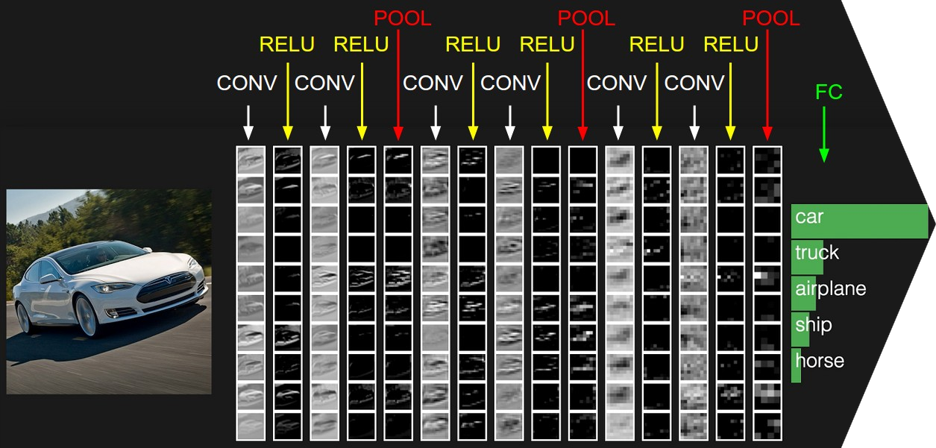
\includegraphics[scale=0.65]{cnn-overview.png}
                        \caption{Long Short-Term Memory Unit \cite{cs231n2023}}
                        \label{cnn-overview-fig}
            
                    \end{center}
                    
                \end{table}
    

                What is a convolutional layer exactly? The four important parts are the filter, kernel, stride, and padding. 
                These are the parameters that will determine how the convolution is performed. 
                First, the number of filters are chosen, also known as output filters, 
                and they determine how many times the image gets passed through the process. 
                One filter means one pass through and one output tensor, while 10 filters mean ten pass throughs and 10 output tensors. 
                The next choice is the size of the filter, which is known as the kernel. 
                An example kernel size is (3,3,3) and this works just like image dimensions, 
                where the height is 3, the width is 3, and the RGB channels are 3. 
                The kernel in the example can be visualized as something that slides over the image 
                and only focuses on a 3-by-3 area at a time. Adding on to the previous example, if the model has 10 filters, 
                then that means there would be 10 output tensors, but that doesn’t mean the output tensor shape would be (3, 3, 3). 
                One needs the last two parameters, stride, and padding, to calculate the output tensor shape. 
                The stride is a number that tells the kernel how many pixels it should move at a time over the image. 
                A stride of one means the kernel moves across the image space 1 pixel at a time. 
                The last parameter padding, or zero-padding, tells the model how many zeros to place around the image 
                so that no vital information is lost when the kernel slides over the image. With the parameters decided, 
                one can now calculate the output volume size or shape of the output tensor.
                
                \textbf{Output Volume Size Equation \cite{cs231n2023}:}
                
                \begin{large}
                    
                    \[ \textnormal{V} = \frac{W - F + 2P}{S} + 1    \]

                \end{large}

                \noindent Where W := input volume size, F := receptive field size (kernel), P := amount of zero padding, 
                and S := stride of kernel

                The convolutional layer is not the only new layer added in a CNN. 
                The layer that often proceeds a convolutional layer is a pooling layer, or in the case of my model, a max pooling layer.
                The CNN and pooling layers work hand in hand to capture the most important parts of an image. 
                Pooling is also known as downsampling and this is where a lower resolution version of an input signal is created. 
                This method is used to retain the large or important structural elements 
                without the fine detail that may not be as useful \cite{brownlee2020}. 
                The outputs of the convolutional layers record the precise position of features 
                but following small movements in the position of the feature, like a cat head slightly turned, 
                will result in worse predictions, so max pooling is utilized, 
                where only the highest value in every feature map or output filter goes on to the next layer. 
                It can be noted that another pooling method, average pooling, can be used. 
                It functions the same but averages the values in the feature patch.
                
                \begin{table}[h]
            
                    \begin{center}
    
                        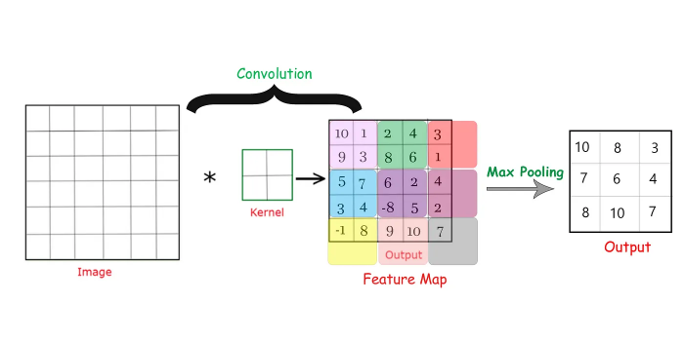
\includegraphics[scale=0.9]{maxpooling.png}
                        \caption{Maxpooling Example \cite{kumar2021} Credit: Codicals}
                        \label{maxpool-fig}
            
                    \end{center}
                    
                \end{table}

                \textbf{Max Pooling Function:}
            
                \begin{large}
                    
                    \[ \textnormal{M} = max(f_i)  \]

                \end{large}

                \noindent for i = 1, ... , F feature map patches


            \subsubsection{Rectified Linear Units}

                As stated earlier, the activation function simply tells the neuron to ‘fire’ or ‘rest’ 
                which in the case of the activation function I used, rectified linear unit function or ReLU, 
                the value returned is either 0 if $ x < 0 $ or x if $ x > 0 $ \cite{agarap2019}. 
                ReLU is used as an activation function for a few key reasons. First, the simple nature of the function, 
                f(x) = max(0,x), eliminates complex calculations and reduces the processing demands. 
                This is especially important in convolutional layers where the amount of parameters can skyrocket 
                and increase the time needed to learn. This works in practice by promoting sparsity in the model 
                and sparsity refers to the scenario where most of the cell entries in a matrix, 
                or in this case tensor, are zero \cite{giskard}.
                
                \textbf{Rectified Linear Units (ReLU):}
            
                \begin{large}
                    
                    \[ f(x) = x^+ = max(0, x) = \frac{x + \vert x \vert}{2} = 
                    \left \{^{\textnormal{x if $x > 0$}}_{\textnormal{0 otherwise}} \right. \]

                \end{large}

                \begin{table}[h]
            
                    \begin{center}
    
                        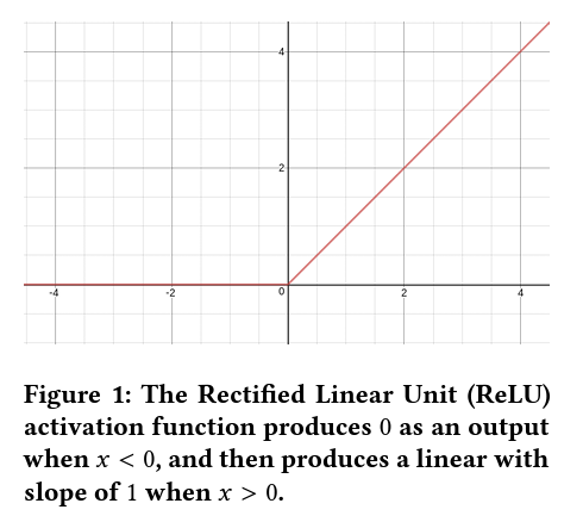
\includegraphics[scale=0.8]{relu.png}
                        \caption{Rectified Linear Unit \cite{agarap2019}}
                        \label{relu-fig}
            
                    \end{center}
                    
                \end{table}            

                
            \subsubsection{Cross-Entropy}
                
                The next important topic to cover is the loss function used since the learning process can only happen 
                if the model has a loss function to calculate the error. 
                The loss function in the models I built was the cross-entropy loss function. 
                These functions, used in classification problems, calculate how accurate the machine learning 
                or deep learning model is by defining the difference between the estimated probability 
                with the desired outcome \cite{365team2023}. These functions come in two versions, 
                one for binary classification and one for categorical classification. 
                My model uses categorical cross-entropy because it is a multi-class classification problem, 
                which means there is only one correct class per x input or image. Had I evaluated if multiple graphs were in an image,
                then it would become a multi-label classification problem, so the final prediction vector would have
                a dimensionality of the number of classes, but each element in the vector could be 0 or 1 depending 
                if the image contains two classes \cite{gomez2018}. For example, if an image had two graphs with one uniform distribution 
                and one normal distribution, then it would look like [0, 0, 1, 1] 
                (classes sorted alphabetically: exp, lognorm, norm, unif). 

                \textbf{Binary Cross-Entropy Function:}

                \begin{large}
                    
                    \[ BCEL = - \frac{1}{N} \sum_{i=1}^N (y_i \cdot log(p_i) + (1 - y_i) \cdot log(1-p_i)) \]

                \end{large}

                \textbf{Categorical Cross-Entropy Function:}
                
                \begin{large}
                    
                    \[ CCEL = - \frac{1}{N} \sum_{i=1}^N \sum_{j=1}^C (y_{i,j} \cdot log(p_{i,j})) \]

                \end{large}

                \noindent Where N := number of rows \newline
                C := number of classes \newline
                y := indicator if class label j is the correct clasification for observation i \newline
                p := predicted probability observation i is of class j

            \subsubsection{Adam Optimizer}

                To wrap up this section over CNNs, the optimizer used to minimize the loss function needs to be mentioned. 
                The optimizer is called gradient descent and it can be described as a first-order iterative algorithm 
                for finding a local minimum of a differentiable multi-variable function. 
                This is apposed to gradient ascent where the algorithm tries to find the local maximum. 
                This can be visually imagined as a rock falling from the mountain side 
                where it will stop once it hits the lowest point or if it gets stuck in a low point between two high points -- 
                which will tried to be avoided. The models use the Adam Optimizer and that is “…an algorithm 
                for first-order gradient-based optimization of stochastic objective functions, based on adaptive estimates 
                of lower-order moments \cite{kingma2015}.” The parameters used are alpha, beta1, beta2, and epsilon. 
                Alpha is also known as the learning rate and determines the stepsize, 
                and is usually very small at around 0.001, which is important, 
                because the algorithm shouldn’t skip over the local minimum. 
                The major advantages of the Adam optimizer are that it only requires first-order gradients 
                and has relatively little memory requirements.

                \begin{table}[ht]
                
                    \begin{center}

                        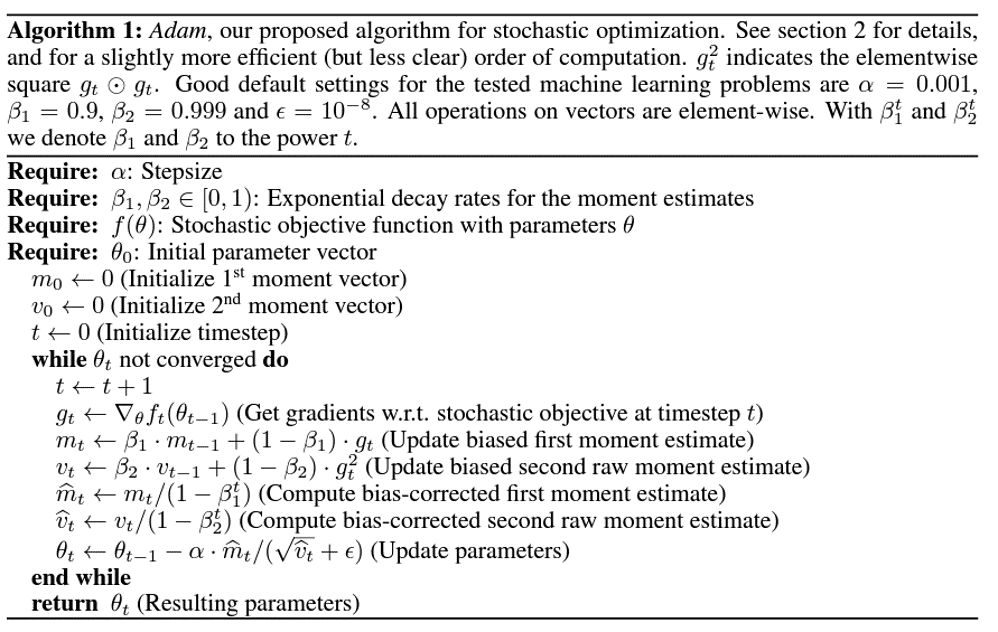
\includegraphics[scale=0.9]{adam-opt.png}
                        \caption{Adam Optimizer Algorithm \cite{kingma2015}}
            
                    \end{center}
                    
                \end{table}


        \subsection{Python, Keras, and Libaries}
                
            The implementation of this project wouldn’t be possible without the various tools used. 
            I’ll describe them all briefly and list out the versions used for the sake of reproducibility in Visual \ref{py-versions}. 
            TensorFlow \cite{abadi2016-tensorflow} is an end-to-end platform for building machine learning models 
            and that works with Keras \cite{chollet2015-keras}, which is a deep learning API written in Python connected to TensorFlow, 
            to create all of the models in this project. 
            Python comes with a plethora of libraries to make working with data and images easier. 
            First there is NumPy \cite{harris2020-numpy} -- a math library with powerful ndarrays. 
            Then there is pandas \cite{reback2020-pandas} \cite{mckinney2010-pandas} 
            which allows for the creation and manipulation of dataframes, which themselves are made up of NumPy’s arrays. 
            The next important library is Matplotlib \cite{hunter2007-matplotlib} 
            where all of the generated graphs used in the models were plotted. 
            Lastly, one of the most important libraires for image classification using TensorFlow 
            and Keras is Pillow \cite{clark2015pillow} since it allows the user to manipulate individual pixels of an image using Python. 
            The PIL Image is a class that can be used and returned using TensorFlow.
                
            \begin{table}[htp]

                \begin{center} 

                \scalebox{1.2}[1.2]{
                \begin{tabular}{ | c | c | }
                \hline
                \textbf{Library}    &       \textbf{Versions} \\
                \hline
                python              &       3.10.13 \\ 
                tensorflow          &       2.10.0 \\
                numpy               &       1.26.0 \\
                pandas              &       2.1.1 \\
                matplotlib          &       3.8.0 \\
                pillow              &       10.0.1 \\
                
                \hline
                \end{tabular}
                }

                \caption{Python und Library Versions}
                \label{py-versions}

                \end{center}

            \end{table}
       

        \subsection{Simplified Graph Classifier}

            In total, four simple graph classifiers were created -- each with a specific purpose of evaluation in mind. 
            The idea behind them was to create a base assumption that the graphs I generated can be considered a realistic dataset 
            one could get if they scraped from various sources. 
            The main goal is to be able to classify graphs into their probability distribution, 
            but this step acts as a bridge and quality assurance for the generated graph dataset 
            which will be used in the distribution graph classifiers. 
            Each model has a specific name consisting of acronyms to distinguish itself: 
            CIFAR is the natural images, SCP is the scraped graphs, GEN stands for the generated graphs, 
            and 1 indicates the model structure. This results in the four models: CIFAR\_SCP\_1, CIFAR\_GEN\_1, GEN\_SCP\_1, 
            and CIFAR\_GEN\_SCP\_1. The model struture for all classifiers is shown by layer in Visual \ref{model-layer-info}.

            \begin{table}[htp]

                \begin{center} 

                \scalebox{0.9}{
                \begin{tabular}{ | l | l | l | }
                \hline
                \textbf{Layer} &  \textbf{Type}     &  \textbf{Parameters}    \\
                \hline
                1              &  Rescaling         &  (1.0/255, input\_shape = (H, W, 3))                \\ 
                2              &  Conv2D            &  (filter\_count = 16, kernal\_size = 3, padding='same', activation = 'relu')   \\
                3              &  MaxPooling2D      &  none                        \\
                4              &  Conv2D            &  (32, 3, 'same', 'relu')                        \\
                5              &  MaxPooling2D      &  none                       \\
                6              &  Conv2D            &  (64, 3, 'same', 'relu')                           \\
                7              &  MaxPooling2D      &  none                           \\
                8              &  Flatten           &  none                            \\
                9              &  Dense             &  (units = 128, 'relu')                            \\
                10             &  Dense             &  (number\_of\_classes = 4)                            \\
                
                \hline
                \end{tabular}
                }

                \caption{Model 1 Layer Information}
                \label{model-layer-info}

                \end{center}

            \end{table}

            \begin{table}[htp]

                \begin{center} 

                \scalebox{1.2}{
                \begin{tabular}{ | c | c | c | }
                \hline
                \textbf{Model Info}    &       \textbf{CIFAR\_SCP\_1}     &       \textbf{CIFAR\_GEN\_1} \\
                \hline
                x                      &       32x32 images               &       32x32 images \\ 
                y                      &       [graph, natural]           &       [graph, natural] \\
                total                  &       17,753                     &       18,000 \\
                train                  &       14,203                     &       14,400\\
                val                    &       3,550                      &       3600 \\
                model                  &       1                          &       1 \\
                
                \hline
                \end{tabular}
                }

                \caption{Model Information for classifying graphs from natural images}
                \label{cifar-graphs-1}

                \end{center}

            \end{table}


            The first model created aims to classify natural images from the scraped graphs. 
            This answers the first basic question: how easily can the model distinguish a natural image from a graph image? 
            The desired outcome would have a high accuracy since graphs have many combinations of characteristics 
            that won’t be found in natural images, for example grid lines, large areas of only one color and surrounding text. 
            One can imagine a natural image with some of these features, but this would be a small number of instances. 
            
            The second model, much like the first one, answers the question: 
            are the generated graphs distinguishable from the natural images as well? 
            This was the first test for the generated graphs and much like the first model, 
            should have achieved high accuracy. The main question here would be the difference in accuracy between CIFAR\_SCP\_1 
            and CIFAR\_GEN\_1 since a higher accuracy in the former would indicate 
            that my generated graphs have some similarities with natural images that are not apparent in the scraped graphs. 
            This could be turned around and a much higher accuracy in CIFAR\_GEN\_1 could indicate 
            that one of my original theories about the scraped dataset could be correct 
            and that is the ‘graph-like’ nature of the images in the scraped dataset which are more artistic 
            or non-numerical representations of graphs. 
            In Visual \ref{cifar-graphs-1}, one can see that the input in CIFAR\_SCP\_1 and CIFAR\_GEN\_1 are balanced.
                        
            GEN\_SCP\_1 was a major test of the simple graph classifier 
            since it will have indicated if my generated graphs were randomized enough to simulate what a bunch of scraped graphs would be.
            The desired outcome here would be a lower accuracy of around 50 percent to show the interchangeability of the two datasets. 
            A high accuracy would indicate the need to randomize the generated graphs more and put them through more preprocessing steps.
                        
            Lastly, all of the datasets were used in a model to classify them as natural, generated, or scraped. 
            The outcome of this would not be as important as the first three, 
            but it would have reinforced the previous intermediate conclusions about the nature of the datasets. 
            A very high accuracy would have meant all datasets are highly distinguishable from one another 
            and point towards tweaking the generated graphs. The information for GEN\_SCP\_1 and CIFAR\_GEN\_SCP\_1
            can be seen in Visual \ref{cifar-gen-scp-1}.
            
            \begin{table}[htp]

                \begin{center} 

                \scalebox{1.2}{
                \begin{tabular}{ | c | c | c | }
                \hline
                \textbf{Model Info}    &       \textbf{GEN\_SCP\_1}       &       \textbf{CIFAR\_GEN\_SCP\_1} \\
                \hline
                x                      &       32x32 images               &       32x32 images \\ 
                y                      &       [generated, scraped]       &       [generated, natural, scraped] \\
                total                  &       15,753                     &       25,753 \\
                train                  &       12,603                     &       20,603\\
                val                    &       3,150                      &       5,150 \\
                model                  &       1                          &       1 \\
                
                \hline
                \end{tabular}
                }

                \caption{Model Information for classifying generated from scraped graphs}
                \label{cifar-gen-scp-1}

                \end{center}

            \end{table}

         
        \subsection{Distribution Graph Classifier}

            The core of the project was being able to create a model that can classify graphs of four different probability distributions 
            and they, like the simple graph classifiers, have specific naming conventions. 
            DIST indicates that they are the distribution classifiers. Number x number specifies the dimensions of the image (width x height). 
            The 1 indicates like earlier the first model structure. The three models are as follows: 
            DIST\_32x32\_1, DIST\_115x86\_1, and DIST\_153x115\_1. It is important to note that dimensions are reversed in TensorFlow 
            and the shape of the image is (height, width, rgb).
            
            \begin{table}[htp]

                \begin{center} 

                \scalebox{0.9}{
                \begin{tabular}{ | c | c | c | c | }
                \hline
                \textbf{Model Info} &  \textbf{DIST\_32x32\_1}      &  \textbf{DIST\_115x86\_1}    &  \textbf{DIST\_153x115\_1} \\
                \hline
                x                   &  32x32 images                 &  115x86 images               &  153x115 images \\ 
                y                   &  [exp, lognorm, norm, unif]   &  [exp, lognorm, norm, unif]  &  [exp, lognorm, norm, unif] \\
                total               &  8,000                        &  8,000                       &  8,000 \\
                train               &  6,400                        &  6,400                       &  6,400 \\
                val                 &  1,600                        &  1,600                       &  1,600 \\
                model               &  1                            &  1                           &  1 \\
                
                \hline
                \end{tabular}
                }

                \caption{Model Information for all distribution graph classifiers}
                \label{dist-dims-1}

                \end{center}

            \end{table}

            The images used, total number of images, training images, validation images, 
            and model structure are all the same, except for the dimensions of the image and that can be seen in Visual \ref{dist-dims-1}.
            The reason for this is how much information is lost when the image is 32x32. 
            It was easy to assume that the model would perform poorly when the density function line almost completely disappears. 
            My solution was to increase the dimensions and thereby its quality. 
            The classes, y target, are as previously stated: exp, lognorm, norm, and unif.
        
    \section{Results}
    
        \subsection{Simple Graph Classifiers}

            The first measure of all of the models were the training and validation accuracy and training and validation loss. 
            The caveat here is the training validation shouldn’t be much higher than the validation accuracy 
            because that indicates overfitting and future poor performance with untrained images. 
            CIFAR\_SCP\_1 performed as expected and reached a 97.55 percent validation accuracy after 3 epochs. 
            Subsequently, the CIFAR\_GEN\_1 performed slightly better with a final 99.89 percent validation accuracy after 3 epochs. 
            Because of the high validation accuracy after 3 epochs, I felt it was unnecessary to increase this parameter more. 
            The crucial model, GEN\_SCP\_1, achieved an accuracy of 99.21 percent, 
            which as I mentioned, is the undesired outcome. This points to the previous hypothesis that the generated graphs 
            and scraped graphs are so different that they can be considered disjunct subsets in the set of all graphs. 
            This would mean the usability of models trained with the generated graphs are extremely limited in their capacity. 
            The ramifications of this result indicate the need to tweak the programs 
            that generate the graphs and the addition of preprocessing techniques. 
            I’ll remark more on these additional techniques in the ‘Conclusions and Further Research’ section. 
            The last simple graph classifier model, CIFAR\_GEN\_SCP\_1 performed 
            how the earlier models indicated with a 98.12 percent validation accuracy.

            \begin{table}
            
                \begin{center}

                    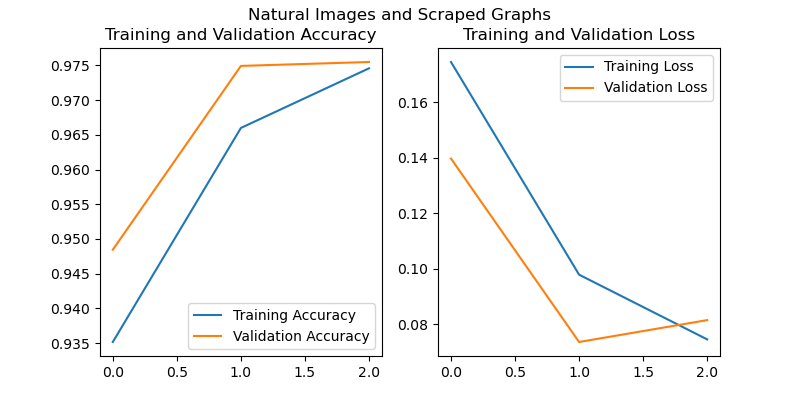
\includegraphics[scale=0.8]{CIFAR_SCP_1_HIST_RESULTS.png}
                    \caption{CIFAR\_SCP\_1 Training and Validation Accuracy and Loss}
                    \label{cifar-scp-acc-loss}
        
                \end{center}
                
        
            
                \begin{center}

                    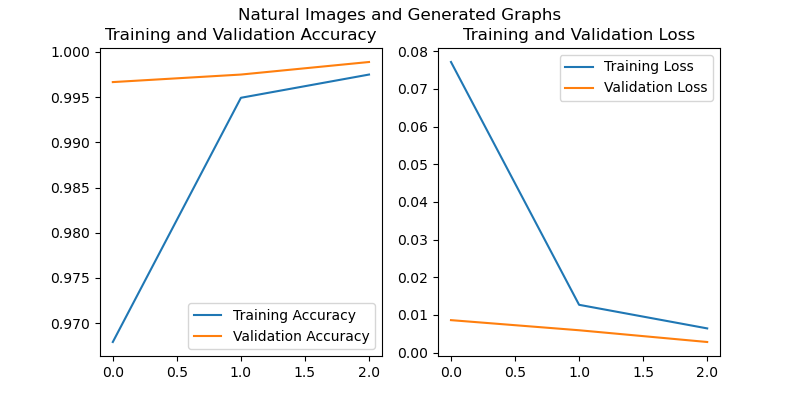
\includegraphics[scale=0.8]{CIFAR_GEN_1_HIST_RESULTS.png}
                    \caption{CIFAR\_GEN\_1 Training and Validation Accuracy and Loss}
                    \label{cifar-gen-acc-loss}
        
                \end{center}

            \end{table}

            \begin{table}
            
                \begin{center}

                    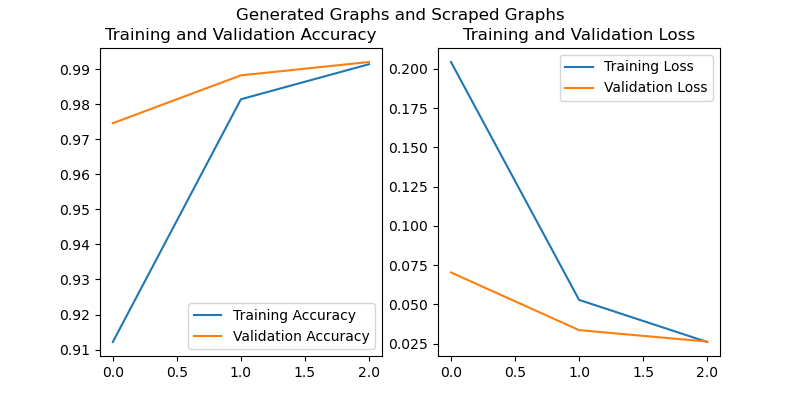
\includegraphics[scale=0.8]{GEN_SCP_1_HIST_RESULTS.png}
                    \caption{GEN\_SCP\_1 Training and Validation Accuracy and Loss}
                    \label{gen-scp-acc-loss}
        
                \end{center}
                
        
            
                \begin{center}

                    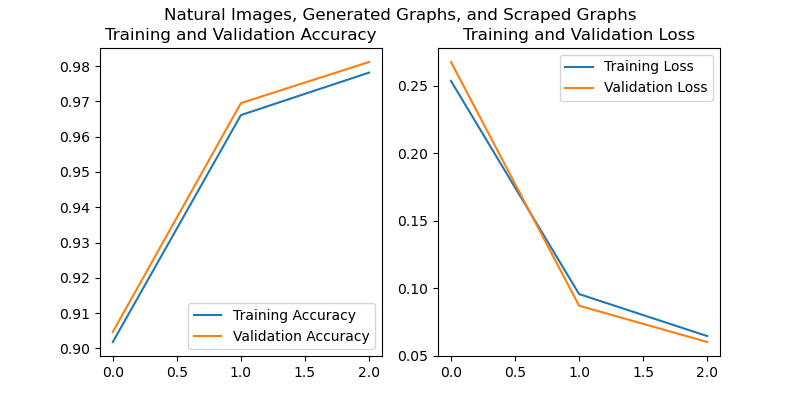
\includegraphics[scale=0.8]{CIFAR_GEN_SCP_1_HIST_RESULTS.png}
                    \caption{GEN\_SCP\_1 Training and Validation Accuracy and Loss}
                    \label{cifar-gen-scp-acc-loss}
        
                \end{center}
                
            \end{table}


            In order to properly evaluate the models, the accuracy and loss were not enough as indicators alone. 
            To this end, I saved all of the models and fed in the graph images they have not seen yet. 
            The models simply classified each image as natural or graph. First, I put the generated graphs in CIFAR\_SCP\_1. 
            The perfect outcome should be 100 percent since all 8,000 images are graphs. 
            The accuracy in this evaluation was 80.94 percent. 
            This could be much better but considering the high accuracy from GEN\_SCP\_1, 
            these graphs are not very similar. Next, the scraped graphs were put into CIFAR\_GEN\_1 
            and, like the above evaluation, should have a perfect accuracy of 100 percent. 
            The accuracy dropped even lower to 37.22 percent which is far from ideal. 
            What does this mean exactly? When graphs from the scraped dataset are put into the CIFAR\_GEN\_1, 
            it classifies most of them as natural images. 
            This outcome strengthens a hypothesis that quite a lot of scraped graphs are ‘graph-like’ 
            and are more similar to natural images. As the generated graphs are the main focus, 
            I took a deeper look at the falsely classified generated graphs in CIFAR\_SCP\_1. 
            The misclassifications were spread out pretty evenly, 
            but the graphs with uniform distribution were most often classified as natural images.
            The counts can be seen in Visual \ref{mis-gen-in-cifar-scp-1-chart} 
            and some examples of misclassified graphs are shown in Visual \ref{mis-gen-in-cifar-scp-1-examples}.
            
            \begin{table}
            
                \begin{center}

                    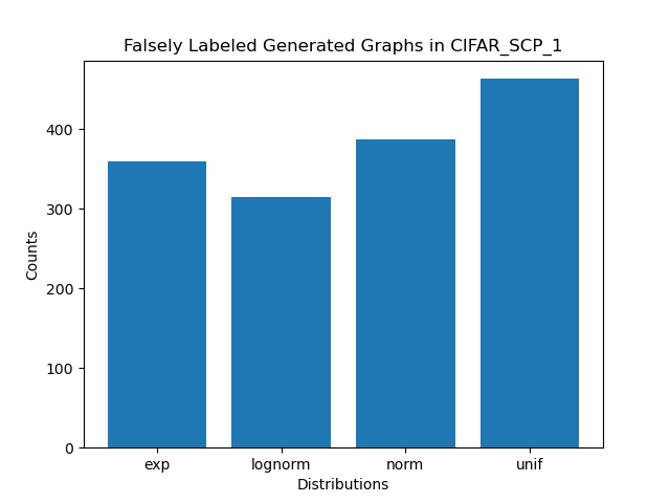
\includegraphics[scale=0.7]{misclassified-gen-in-cifar-scp-1.png}
                    \caption{Misclassified generated graphs in CIFAIR\_SCP\_1}
                    \label{mis-gen-in-cifar-scp-1-chart}
        
                \end{center}
                
            \end{table}

            \begin{table}
                \begin{center}
                
                    \begin{tabular}{ c  c }

                        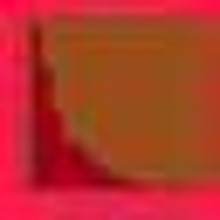
\includegraphics[scale=0.74]{mis-as-nat-exp-20.jpg} & 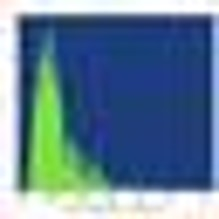
\includegraphics[scale=0.74]{mis-as-nat-lognorm-544.jpg} \\
                
                        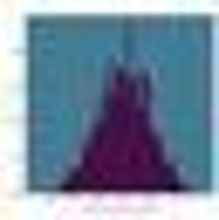
\includegraphics[scale=0.74]{mis-as-nat-norm-695.jpg} & 
\includegraphics[scale=0.74]{mis-as-nat-unif-352.jpg} \\

                    \end{tabular}

                    \caption{Examples of misclassified generated graphs as natural images}
                    \label{mis-gen-in-cifar-scp-1-examples}

                \end{center}

            \end{table}


        \subsection{Distribution Graph Classifiers}

       
            Just as before, I’ll first cover the training and validation accuracy 
            and training and validation loss of each distribution graph classifier first. 
            I’ll start with image data from the lowest dimension to the highest. 
            The DIST\_32x32\_1 ran for 10 epochs since the model originally struggled to classify the graphs in only 3 epochs 
            like the simple graph classifiers. This is a reasonable change in parameters 
            since it is no longer a binary classification problem but a multi-class classification problem. 
            After training it reached an accuracy of 79.25 percent validation accuracy. 
            At an image size of 32x32 pixels this accuracy surprised me, 
            especially when you can see that after one epoch the validation accuracy was already above 60 percent. 
            Increasing the quality, or dimensions, of the image greatly increased accuracy. 
            The DIST\_115x86\_1 was able to achieve a validation accuracy of 93.00 percent after 10 epochs. 
            However, there is a diminishing return in regard to image quality 
            since the validation accuracy only improved by 0.5 percent to 93.5 percent in the model DIST\_153x115\_1. 
            Overall, the results are promising, but they require an evaluation to see where the graphs are getting misclassified. 
            The validation accuracy of DIST\_115x86\_1 and DIST\_153x115\_1 are hanging around 93 percent, 
            so the question becomes what are the images that are not getting classified correctly. 
            
            \begin{table}
            
                \begin{center}

                    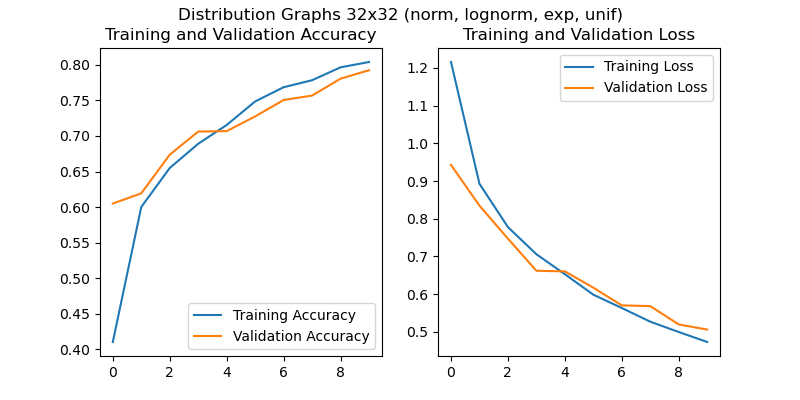
\includegraphics[scale=0.6]{DIST_32x32_1_HIST_RESULTS.png}
                    \caption{DIST\_32x32\_1 Training and Validation Accuracy and Loss}
                    \label{dist-32-32-val-loss}
        
                \end{center}
                
        
            
                \begin{center}

                    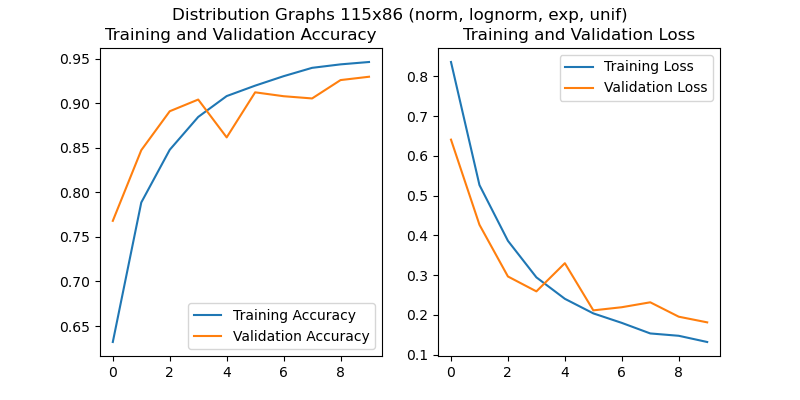
\includegraphics[scale=0.6]{DIST_115x86_1_HIST_RESULTS.png}
                    \caption{DIST\_115x86\_1 Training and Validation Accuracy and Loss}
                    \label{dist-115-86-val-loss}
        
                \end{center}

            
                \begin{center}

                    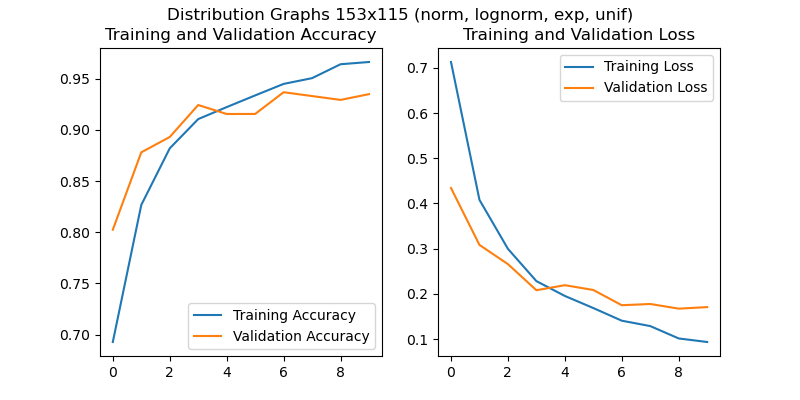
\includegraphics[scale=0.6]{DIST_153x115_1_HIST_RESULTS.png}
                    \caption{DIST\_153x115\_1 Training and Validation Accuracy and Loss}
                    \label{dist-153-115-val-loss}
        
                \end{center}
             
                
            \end{table}

            After the training was finished, I saved all the models and fed all 8,000 graphs into the DIST\_153x115\_1 for evaluation. 
            I decided to stick with evaluating one model since doing the same process for all would have been redundant 
            and not given me further insights into the data and model performance. 
            I chose DIST\_153x115\_1 instead of the other two because it performed slightly better 
            but using DIST\_115x86 would have been viable as well. The saved DIST\_153x115\_1 model performed well in the evaluation 
            by accomplishing an accuracy of 96.54 percent. That means there were a total of 270 misclassifications out of 8,000 images,
            and the results can be seen in Visual \ref{mis-all-count-in-dist} and Visual \ref{counts-all-gen-dist}.
            The probability distribution with the most misclassifications was the exponential distribution at 149, 
            while the lowest was the uniform distribution with only 6 misclassifications. 
            Why were graphs with an exponential distribution most often labelled incorrectly 
            and by such a wide margin? A closer look at the data in Visual \ref{mis-all-count-in-dist} shows that almost all of the exponential distribution graphs 
            that were misclassified where misclassified as the log-normal distribution. 
            When one looks at the images in question then it is easier to see why that is the case, 
            but it is still noteworthy how high the accuracy is despite the similarities. 
            There were 2,000 exponential distribution graphs and only 147 were labeled as log-normal distribution 
            which still indicates a strong performance.

            \begin{table}

                
                
                \begin{center}
                    
                    \begin{tabular}{ c  c }

                        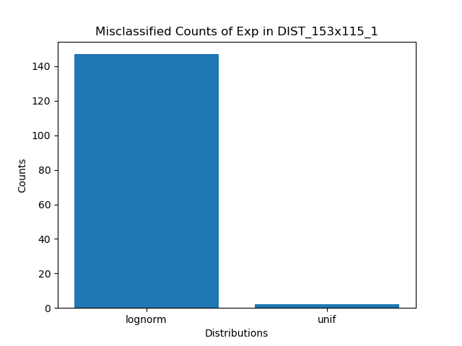
\includegraphics[scale=0.63]{mis-exp-count-in-dist.png} & 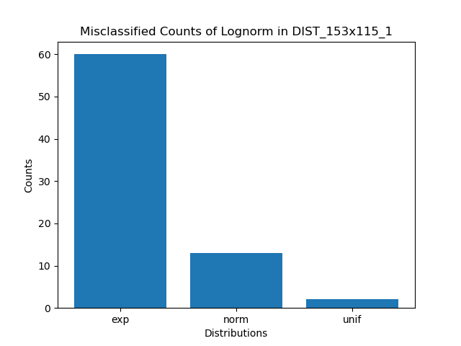
\includegraphics[scale=0.63]{mis-lognorm-count-in-dist.png} \\
                
                        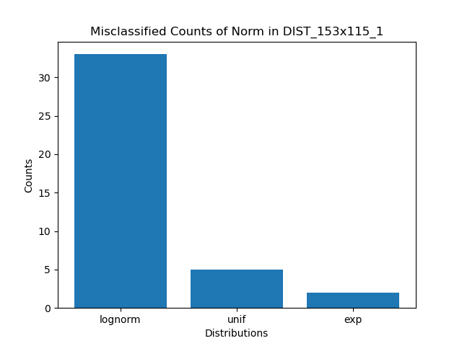
\includegraphics[scale=0.63]{mis-norm-count-in-dist.png} & 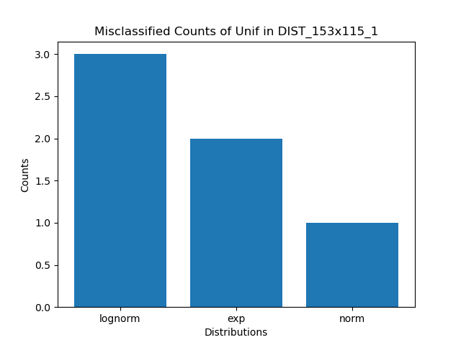
\includegraphics[scale=0.63]{mis-unif-count-in-dist.png} \\

                    \end{tabular}

                    \caption{Counts of misclassified generated graphs in DIST\_153x115\_1}
                    \label{mis-all-count-in-dist}

                \end{center}

            \end{table}

            \begin{table}

                \begin{center}

                    \begin{tabular}{| l | c | c | c | c |}

                        \hline
                        \textbf{Prediction}   &    \textbf{Exp}   &   \textbf{Lognorm}   &    \textbf{Norm}    &    \textbf{Unif} \\
                        \hline
                        True                  & 1,851             & 1,925                & 1,960               & 1,994 \\
                        False                 & 149               & 75                   & 40                  & 6 \\

                        \hline

                    \end{tabular}

                    \caption{Counts of correctly and falsely classified generated graphs in DIST\_153x115\_1}
                    \label{counts-all-gen-dist}

                \end{center}

            \end{table}
            
            In order to understand the results better and have a clear record of all the evaluations, 
            I created CSVs with relevant information. They include the ending prediction weight for each class, 
            the true or false prediction, the file name, the max weight, and the label based on the max.
            With the results readily available, it was easy to see some patterns. 
            In my earlier caveats, it was stated that the normal and log-normal distribution can look quite similar 
            if given the right parameters and that plays out when one looks at 
            how the model misclassified some normal distribution graphs as log-normal. 
            Also, from the earlier section about the generated graphs, 
            I mentioned the so-called ‘duds’ and that comes up in the evaluations as well. 
            All of the uniform distribution graphs misclassified can be considered ‘duds’ in that they appear blank.

            \begin{table}

                \scalebox{0.75}{

                    \begin{tabular}{l | l | l | l | l | l | l | l | l}
                        \hline
                        \textbf{exp}         & \textbf{lognorm}     & \textbf{norm}         & \textbf{unif}       & \textbf{max}       & \textbf{file\_name}         & \textbf{actual}  & \textbf{label}   & \textbf{prediction} \\
                        \hline
                        -4.1661463  & 8.161812    & 0.9788155    & -10.229221 & 8.161812  & exp\_12.jpeg       & exp     & lognorm & False      \\
                        3.8511171   & 4.496506    & -3.405139    & -5.2995405 & 4.496506  & exp\_2.jpeg        & exp     & lognorm & False      \\
                        5.872565    & 11.971514   & -6.275291    & -12.128517 & 11.971514 & exp\_20.jpeg       & exp     & lognorm & False      \\
                        9.207311    & 10.764248   & -11.954131   & -5.3854074 & 10.764248 & exp\_3.jpeg        & exp     & lognorm & False      \\
                        -5.917483   & 15.367903   & -4.7242074   & -5.200668  & 15.367903 & exp\_5.jpeg        & exp     & lognorm & False      \\
                        6.1337843   & 6.400875    & -5.021023    & -7.4242744 & 6.400875  & exp\_8.jpeg        & exp     & lognorm & False      \\
                        0.51164746  & 8.585008    & -3.2878444   & -6.293257  & 8.585008  & exp\_9.jpeg        & exp     & lognorm & False      \\
                        -2.7664876  & 8.546496    & 0.33398134   & -9.835137  & 8.546496  & exp\_hand\_0.jpeg  & exp     & lognorm & False      \\
                        -13.257631  & 5.875923    & -2.4565024   & 7.38458    & 7.38458   & lognorm\_0.jpeg    & lognorm & unif    & False      \\
                        3.7302907   & 2.0135944   & -0.048096493 & -11.51519  & 3.7302907 & lognorm\_5.jpeg    & lognorm & exp     & False      \\
                        -14.977435  & 3.678837    & 1.5030111    & 1.7347182  & 3.678837  & norm\_1.jpeg       & norm    & lognorm & False      \\
                        -0.31633773 & 5.5405626   & 1.6448251    & -18.00231  & 5.5405626 & norm\_11.jpeg      & norm    & lognorm & False      \\
                        -14.40909   & 10.438942   & 7.7604384    & -26.327517 & 10.438942 & norm\_13.jpeg      & norm    & lognorm & False      \\
                        -5.3496103  & 7.2749767   & 1.1707792    & -6.384265  & 7.2749767 & norm\_14.jpeg      & norm    & lognorm & False      \\
                        -6.992462   & 7.189061    & 4.9432883    & -15.288852 & 7.189061  & norm\_15.jpeg      & norm    & lognorm & False      \\
                        -4.783489   & 4.332031    & 3.8387465    & -14.778937 & 4.332031  & norm\_19.jpeg      & norm    & lognorm & False      \\
                        -23.318886  & 12.883771   & -0.8641091   & 5.143599   & 12.883771 & norm\_4.jpeg       & norm    & lognorm & False      \\
                        -25.816198  & 16.998684   & 4.5914965    & -9.728744  & 16.998684 & norm\_8.jpeg       & norm    & lognorm & False      \\
                        -6.6115365  & 7.848427    & 0.57640886   & -4.26034   & 7.848427  & norm\_9.jpeg       & norm    & lognorm & False      \\
                        -0.7095418  & 1.1841375   & -0.53598833  & -1.6236649 & 1.1841375 & unif\_0.jpeg       & unif    & lognorm & False      \\
                        -4.572587   & 5.3358355   & 0.4110088    & -3.925213  & 5.3358355 & unif\_1.jpeg       & unif    & lognorm & False      \\
                        -2.4820209  & -0.05105117 & 2.7819424    & -4.3270063 & 2.7819424 & unif\_10.jpeg      & unif    & norm    & False      \\
                        -4.820385   & 9.742123    & -7.255406    & 6.477165   & 9.742123  & unif\_11.jpeg      & unif    & lognorm & False      \\
                        -0.5606266  & 6.14713     & -2.2170813   & -3.020845  & 6.14713   & unif\_12.jpeg      & unif    & lognorm & False      \\
                        1.1152176   & 1.1827534   & -0.67093164  & -5.319949  & 1.1827534 & unif\_13.jpeg      & unif    & lognorm & False      \\
                        -0.19624099 & 7.653762    & -2.4959579   & -3.569571  & 7.653762  & unif\_14.jpeg      & unif    & lognorm & False      \\
                        -0.46984562 & 5.252478    & -4.9778605   & 1.5037757  & 5.252478  & unif\_16.jpeg      & unif    & lognorm & False      \\
                        -0.20320779 & 4.1991606   & 1.5740888    & -10.120164 & 4.1991606 & unif\_17.jpeg      & unif    & lognorm & False      \\
                        -2.3884668  & 3.9697368   & -0.6534233   & -2.8202808 & 3.9697368 & unif\_2.jpeg       & unif    & lognorm & False      \\
                        1.6306777   & 6.3168035   & -0.7305184   & -8.0671625 & 6.3168035 & unif\_3.jpeg       & unif    & lognorm & False      \\
                        -5.6656113  & 4.946749    & 1.8187       & -6.4847775 & 4.946749  & unif\_4.jpeg       & unif    & lognorm & False      \\
                        -4.4202156  & 3.0252044   & 1.0488026    & -2.0555344 & 3.0252044 & unif\_5.jpeg       & unif    & lognorm & False      \\
                        5.331371    & 4.629284    & -3.9633603   & -6.628367  & 5.331371  & unif\_6.jpeg       & unif    & exp     & False      \\
                        -4.064364   & 4.5016537   & -3.487114    & 3.3282218  & 4.5016537 & unif\_8.jpeg       & unif    & lognorm & False      \\
                        -6.592189   & -0.6548197  & 2.7110033    & -1.7038764 & 2.7110033 & unif\_9.jpeg       & unif    & norm    & False      \\
                        0.5345101   & 0.08001919  & 0.43601054   & -6.1528854 & 0.5345101 & unif\_hand\_0.jpeg & unif    & exp     & False      \\
                        \hline   
                
                    \end{tabular}
                    
                }

                \caption{All Misclassified Images in Final Test Evaluation}
                \label{all-mis-test-eval}

            \end{table}
            
            To wrap up my evaluations and to truly assess my generated graphs and models, 
            I needed to use graphs that have not been used in any model previously. 
            Visual \ref{all-mis-test-eval} contains all images in the final test evaluation that were misclassified.
            To get this, I simply gathered 20 graphs of every distribution type from random sources online 
            and then added one graph of each distribution drawn by hand. 
            I felt this would add some realistic grounding to the final evaluation. 
            Each distribution had 21 graphs, so a total of 84 graphs. 
            The final evaluation accuracy was 59.10 percent and fell in line with my more hopeful expectations. 
            This evaluation is similar to when the scraped graphs where put into CIFAR\_GEN\_1 and if you can remember, 
            the accuracy was only 37.22 percent. So overall, it is a positive development. 
            Just like before the question becomes what was getting misclassified 
            and here is where the results diverged from my original predictions. 
            Almost all of the misclassified graphs were misclassified as log-normal,
            which can be seen in the 'label' column in Visual \ref{all-mis-test-eval}. 
            And if one analyzed this more granularly then one can see 
            that the uniform distribution graphs were overwhelmingly misclassified as log-normal. 
            13 graphs out of the 21 uniform graphs were misclassified as log-normal. 
            It is surprising how 61.90 percent of uniform graphs in the test dataset were misclassified as log-normal 
            since the generated uniform graphs were predicted so accurately in DIST\_153x115\_1.
            I can conclude for now that the model needs more diverse training images to account for the variety in graphs found online
            and more images to train on.
            

        
        \subsection{Conclusions and Further Research}

            As a whole, I can say that the main goals were accomplished. 
            I have a model that can successfully identify graphs from natural images 
            with greater than 98 percent accuracy and another model that can successfully identify my generated graphs 
            with four different distribution types with around 93 percent accuracy. 
            However, when more diverse graphs are included this drops down to 59.10 percent as shown in the 
            final test evaluation and in Visual \ref{all-mis-test-eval}.
            Addendum to these results is the caveat from earlier that the generated graphs could be considered as a disjunct subset, 
            if one considers the scraped graphs to be a genuine sample of possible and currently available graphs. 
            The GEN\_SCP\_1’s high accuracy points towards this theory but a large limiting factor is the small sample size -- 
            only 8,000 generated graphs and 7,753 scraped graphs. 
            Some results that surprised me were that scraped graphs in CIFAR\_GEN\_1 were misclassified as natural images 
            around 63 percent of the time. This could indicate 
            that the generated graphs don’t consider the more chaotic nature of graph design -- 
            this is substantiated by the final test evaluation as well.
            It would be safe to say that the generated graphs are very conservative in appearance. 
            However, this was an original design choice to reduce the amount of variables in the graphs design, 
            like not having two graphs in one image or keeping to the standard of having a complete graph in each image. 
            Many graphs, like the ones in the scraped dataset 
            and the ones I used in the final test evaluation, don’t have any axes, labels, or titles. 
            This enforces the idea that many of the images in SCP and many graphs in general are more ‘graph-like’ 
            and not graphs in a very defined sense.
            Another surprise was the difference in how the uniform distribution graphs were getting misclassified.
            Uniform distribution graphs in DIST\_153x115\_1 were classified accurately around 99 percent of the time, 
            but 20 percent of generated uniform graphs in CIFAR\_SCP\_1 were misclassified as natural images. 
            Why were the graphs easily classified in DIST\_153x115\_1 but not in CIFAR\_SCP\_1? 
            Perhaps graphs with the uniform distribution are unique from the other distribution graphs 
            but not very unique from natural images. The final test evaluation bucked this trend by
            classifying uniform distribution as log-normal for a majority of the graphs.
            However, in the final test evaluation almost all of the misclassified images were
            classified as log-normal, so this might point to an issue with the training images.
            
            \begin{table}[h]

                \begin{center}

                    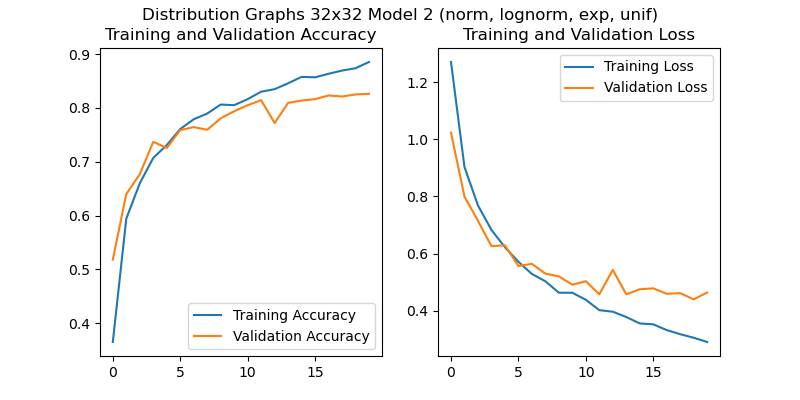
\includegraphics[scale=0.6]{DIST_32x32_2_HIST_RESULTS.png}
                    \caption{DIST\_32x32\_2 Training and Validation Accuracy and Loss}
                    \label{dist-32-32-2-val-loss}
        
                \end{center}
            
            \end{table}

            To conclude I’ll propose some possible changes and improvements to further this line of research. 
            The quickest improvements could simply come from changing the model structure and tweaking the parameters. 
            While I only used one convolutional layer at a time, 
            another common CNN architecture is to stack two convolutional layers before each pooling later. 
            This is strongly encouraged as this allows for more complex features of the input vector to be selected \cite{oshea2015}. 
            Regarding the parameters, I built a second model by doubling the number of filters in the convolution layers. 
            The training and validation accuracy and loss of DIST\_32x32\_2
            are shown in Visual \ref{dist-32-32-2-val-loss} --
            the 2 indicates the second model used.
            There were minor improvements to the validation accuracy of the DIST\_32x32\_1, 
            but the issue of overfitting is seen after 10 epochs. Secondly, one could use more images to train each model. 
            It would be quite easy to generate 20,000 graphs, but that depends on the quality and ‘generalness’ of the graphs. 
            The generated graphs used in this experiment were highly distinguishable from the scraped graphs 
            and that leads to the next change, and that is improving the generated graphs. 
            The scripts that created the graphs can be improved to increase variability, 
            but another way is adding more preprocessing layers. TensorFlow has a host of different methods 
            that change brightness, contrast, crop, flip, and rotation, 
            which would do a good job at simulating the chaotic nature of graphs created by people from all over the world. 
            Finally, the experiment could be further by simply expanding the probability distributions used.
            
            As stated at the beginning, the focus was on identifying and classifying graphs, 
            but it was just the first step in a large picture of identifying, locating, and organizing. 
            To extend a practical use case for this project, one could start using entire reports as input to train the model. 
            In this scenario, pages with graphs on them would be the y target. 
            With the pages identified, they could be returned to the user for quick viewing. 
            From there the model could be expanded to only retrieve the graphs themselves and organize them into types. 
            This would require more advanced techniques, 
            especially those in the field of explainable AI \cite{kamakshi2023}, 
            to target specific parts on a page and be able to extract more information.
        
    
    \printbibliography[heading=bibintoc, title={References}]


\end{document}